% Chapter Template

\chapter{OpenFOAM} % Main chapter title

\label{openfoam} % Change X to a consecutive number; for referencing this chapter elsewhere, use \ref{ChapterX}


\section{UEqn}

.../reactingFoam/UEqn.H:

\begin{verbatim}
MRF.correctBoundaryVelocity(U);
 
 tmp<fvVectorMatrix> tUEqn
 (
     fvm::ddt(rho, U) + fvm::div(phi, U)
   + MRF.DDt(rho, U)
   + turbulence->divDevRhoReff(U)
  ==
     fvOptions(rho, U)
 );
 fvVectorMatrix& UEqn = tUEqn.ref();
 
 UEqn.relax();
 
 fvOptions.constrain(UEqn);
 
 if (pimple.momentumPredictor())
 {
     solve(UEqn == -fvc::grad(p));
 
     fvOptions.correct(U);
     K = 0.5*magSqr(U);
 }
\end{verbatim} 
\vspace{\baselineskip}
The tmp wrapper has to do with optimizing the code for decreasing peak memory usage. Normally when C++ returns an object, it copies the object, returns the copy and deletes the original. This means that for a brief moment you have 2 data objects at the same time, which for complex grids can take a lot of memory. By wrapping large data structures in a tmp<Type> wrapper with a reference to the data, one overwrites the constructor and destructor of the object so that when the object is returned, a copy of the reference is created instead of a copy of the object itself. After returning the reference, the original pointer is dereferenced.
\vspace{\baselineskip}
MRF stands for multiple reference field, and has to do with rotational phenomena like fans and golf balls. The terms involving MRF need not be applied for our purposes.
\vspace{\baselineskip}
Looking at the fvm::ddt(rho, U) term, fvm:: means that it expresses the sought after term $\frac{d \rho \textbf{u}}{dt}$ in an implicit way, returning a matrix of coefficients. This is unlike functions in the fvc$::$ namespace, which return sought after values explicitly (by evaluating source terms or predicted terms).
\vspace{\baselineskip}
First we take a look at the turbulence->divDevRhoReff function. It returns the density times the effective viscous stress contribution to the momentum equation. Its implementation depends on the turbulence model chosen. To keep things simple I will look at the version implemented in linearViscousStress.C:
\vspace{\baselineskip}
\begin{verbatim}
 Foam::linearViscousStress<BasicTurbulenceModel>::divDevRhoReff
 (
     volVectorField& U
 ) const
 {
     return
     (
       - fvc::div((this->alpha_*this->rho_*this->nuEff())*dev2(T(fvc::grad(U))))
       - fvm::laplacian(this->alpha_*this->rho_*this->nuEff(), U)
     );
 }
\end{verbatim}
Alpha\_ is phase fraction, which for single phase solvers like reactionFoam is equal to 1.
\vspace{\baselineskip}
For the viscosity, $\mu_{eff} = \mu_t + \mu$. $\mu_t$ is calculated based on the turbulence model, and $\mu$ is typically read from the input file.
\vspace{\baselineskip}
dev stands for \textbf{deviatory}, and is defined by $dev(A) = A - \frac{1}{3}*tr(A)I$. dev2 is a slight modification, where $dev2(A) = A - \frac{2}{3}*tr(A)I$.
\vspace{\baselineskip}
From this, divDevRhoEff translates into:

\begin{figure}[H]
\centering
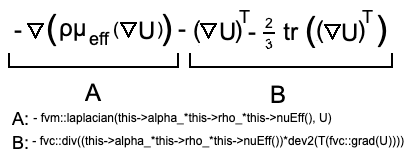
\includegraphics[scale=0.8]{divdevrhoreff}
\end{figure}

In the book (page 23), one equation for the viscous stress in the x-direction is:

\begin{figure}[H]
\centering
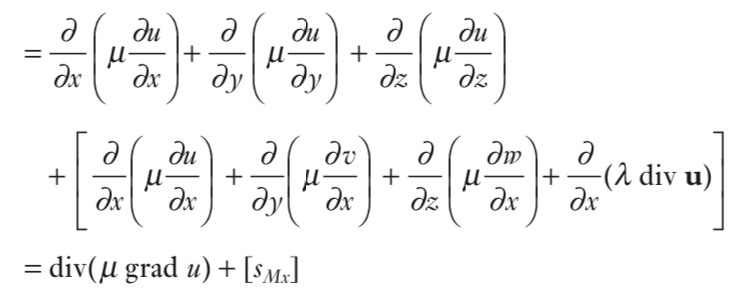
\includegraphics[scale=0.8]{viscous}
\end{figure}

Where $\lambda = -\frac{2}{3}\mu$ (an approximation commonly used for gaseous liquids). Similar equations can be derived for the y- and z-directions.
\vspace{\baselineskip}
For our momentum gradient matrix we have:
\begin{figure}[H]
\centering
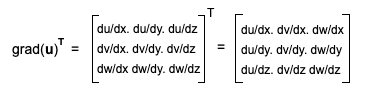
\includegraphics[scale=0.8]{gradUT}
\end{figure}

We can see that the first row of $grad(U)^T$ (corresponding to the shear stress in the x-direction) matches the gradients in the $[S_{Mx}]$ part of the equation.
\vspace{\baselineskip}
The $\frac{d}{dx}$ operator (and corresponding operators for the other directions) in $\frac{d}{dx}(\lambda div(\textbf{u}))$ term makes it so that only the diagonal of $grad(\textbf{u})^T$ is subtracted from.
\vspace{\baselineskip}
Since $div(U)=\frac{du}{dx} + \frac{dv}{dy} + \frac{dw}{dz} tr(grad(U)^T)$ we can now express $[S_{M}]$ (for all three directions) as $div(\mu grad(U)^T - \frac{2}{3} tr( \mu div(U)) = \mu dev2( grad(U)^T)$. $\mu$ can be moved outside of the matrix due to dev being a linear operator.
\vspace{\baselineskip}
We can clearly see this being represented in code through the line
\begin{verbatim}
- fvc::div((this->alpha_*this->rho_*this->nuEff())*dev2(T(fvc::grad(U))))
\end{verbatim}
while the $div(\mu grad(\textbf{u})$ term in the viscous part of the momentum equation is represented by
\begin{verbatim}
- fvm::laplacian(this->alpha_*this->rho_*this->nuEff(), U)
\end{verbatim}
The minus signs come from them being moved from the RHS in the book to the LHS in the solver.
\vspace{\baselineskip}
The multiplication with $\rho$ is in order to convert from kinematic to dynamic viscosity.
\vspace{\baselineskip}
Lastly I'm not sure why the first term is calculated explicitly while the second term is calculated explicitly.
\vspace{\baselineskip}
-----------
\vspace{\baselineskip}
Going back to the momentum equation, if we include the pressure correction (\begin{verbatim}solve(UEqn == -fvc::grad(p)); \end{verbatim} we get the following equation:

\begin{figure}[H]
\centering
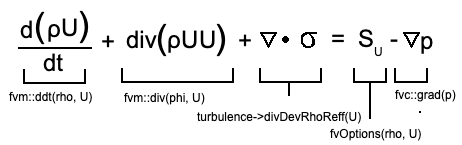
\includegraphics[scale=0.8]{momentumE}
\end{figure}

Where $\sigma$ is the newtonian stress tensor.
\vspace{\baselineskip}
After moving some terms to the RHS, it becomes almost exactly the momentum equation from the book.

\begin{figure}[H]
\centering
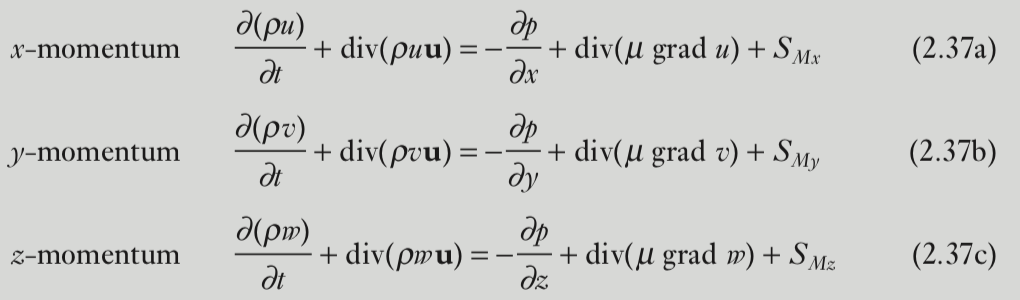
\includegraphics[scale=0.8]{momentumbook}
\end{figure}

UEqn.relax() constrains the magnitude of change in U compared to $U_0$ below a certain value, depending on the relaxation factors specified in fvSolutions.
\vspace{\baselineskip}
fvOptions.constrain(UEqn) adds user-specified boundary conditions (for example, the inlet patch must always have a flow of (3 0 0), or U cannot exceed 200 in magnitude), set in fvOptions.
\vspace{\baselineskip}
Since p was used explicitly in the equation it has not been updated since the last timestep, and does not satisfy the continuity equation with the new U matrix. fvOptions.correct(U) adjusts p with the new U so that the continuation equation is once again satisfied. 
\vspace{\baselineskip}
The line K = 0.5*magSqr(U) sets the kinematic velocity K to $0.5*U^2$.
\vspace{\baselineskip}
Since reactingFoam uses the pimple algorithm, U is not solved fully at every loop iteration, only when pimple.momentumPredictor() = true. For when the predictor is set to false, the velocity is only calculated in the PEqn.C file, at the line:
\vspace{\baselineskip}
U = HbyA - rAU*fvc::grad(p);

\section{pEqn}

.../reactingFoam/pEqn.H:
\begin{verbatim}
    rho = thermo.rho();
 
 volScalarField rAU(1.0/UEqn.A());
 surfaceScalarField rhorAUf("rhorAUf", fvc::interpolate(rho*rAU));
 volVectorField HbyA(constrainHbyA(rAU*UEqn.H(), U, p));
 
 if (pimple.nCorrPiso() <= 1)
 {
     tUEqn.clear();
 }
 
 ...
 
 {
     surfaceScalarField phiHbyA
     (
         "phiHbyA",
         (
             fvc::flux(rho*HbyA)
           + MRF.zeroFilter(rhorAUf*fvc::ddtCorr(rho, U, phi))
         )
     );
 
     MRF.makeRelative(fvc::interpolate(rho), phiHbyA);
 
     // Update the pressure BCs to ensure flux consistency
     constrainPressure(p, rho, U, phiHbyA, rhorAUf, MRF);
 
     while (pimple.correctNonOrthogonal())
     {
         fvScalarMatrix pEqn
         (
             fvm::ddt(psi, p)
           + fvc::div(phiHbyA)
           - fvm::laplacian(rhorAUf, p)
          ==
             fvOptions(psi, p, rho.name())
         );
 
         pEqn.solve();
 
         if (pimple.finalNonOrthogonalIter())
         {
             phi = phiHbyA + pEqn.flux();
         }
     }
 }
 
 #include "rhoEqn.H"
 #include "compressibleContinuityErrs.H"
 
 // Explicitly relax pressure for momentum corrector
 p.relax();
 
 U = HbyA - rAU*fvc::grad(p);
 U.correctBoundaryConditions();
 fvOptions.correct(U);
 K = 0.5*magSqr(U);
 
 if (pressureControl.limit(p))
 {
     p.correctBoundaryConditions();
     rho = thermo.rho();
 }
 
 if (thermo.dpdt())
 {
     dpdt = fvc::ddt(p);
 }
\end{verbatim}

(There is also a pcEqn.H, which will be excecuted if pimple is set to consistent. I will not go through it here.)
\vspace{\baselineskip}
The PEqn.H file first solves the pressure p iteratively and predicts the velocity U in accordance with the PISO loop. Through the momentum equation we can build the velocity coefficient matrix M, where \textbf{MU} = $-\nabla p$. From this the following matrices are defined:
\\\\
A = diag(M) \\
H = AU - MU \\
$rAU = A^{-1}$ \\
rhorAUf = $\rho A^{-1}$ (evaluated at the faces)
HbyA = $A^{-1}H$
phiHbyA = flux(rho*HbyA)
\vspace{\baselineskip}
A represents the pressure contribution from the velocity of a cell.
H represents the pressure contributions from the velocity neighboring cells.
\vspace{\baselineskip}
Let's take a look at the pressure correction loop:

\begin{verbatim}
    while (pimple.correctNonOrthogonal())
     {
         fvScalarMatrix pEqn
         (
             fvm::ddt(psi, p)
           + fvc::div(phiHbyA)
           - fvm::laplacian(rhorAUf, p)
          ==
             fvOptions(psi, p, rho.name())
         );
 
         pEqn.solve();
 
         if (pimple.finalNonOrthogonalIter())
         {
             phi = phiHbyA + pEqn.flux();
         }
     }
\end{verbatim}
The loop will iterate an amount of times based on how orthogonal the matrix is, in order to iteratively calculate the fluxes. For fully orthogonal matrices, it will only execute once. For each iteration, the term fvc::div(phiHbyA) will change, since it is calculated explicitly and depends on p.
\vspace{\baselineskip}
psi = $\psi = \frac{rho}{p}$, meaning the ddt term is basically just $\frac{d \rho}{dt}$
\vspace{\baselineskip}
Note that since we are solving for $\nabla p$, which depends on the flux on cell faces, we are first solving for cell faces rather than cell centers. Because of this, our terms are multiplied by $\rho$ to keep consistency with the continuity equation when calculating the divergence of phiHbyA.
\vspace{\baselineskip}
Solving for the Laplacian term we get:

\begin{figure}[H]
\centering
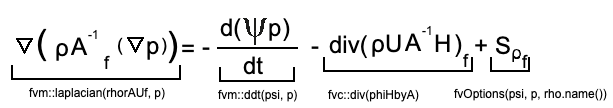
\includegraphics[scale=0.6]{pressurecode}
\end{figure}

This looks similar to the equation at the bottom of page 8 in the "A low-Mach number solver for variable density flows" paper:

\begin{figure}[H]
\centering
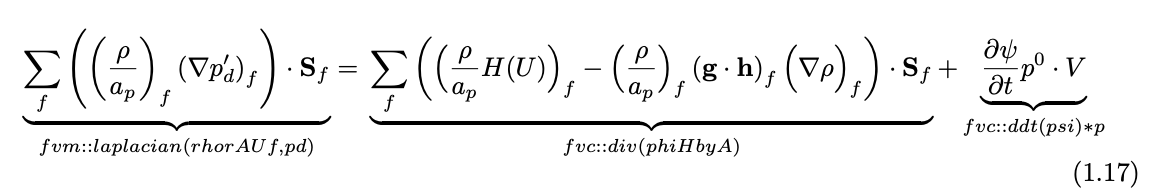
\includegraphics[scale=0.6]{pressuref}
\end{figure}

Since our equation came from the standard reactingFoam solver and not the buoyant one, and since the solver doesn't use a low-mach approximation, the gh term is missing and the pressure terms are slightly different.
\vspace{\baselineskip}
If you follow page 8 of that paper from bottom to top you will find how to derive this discretized version of the equation:

\begin{figure}[H]
\centering
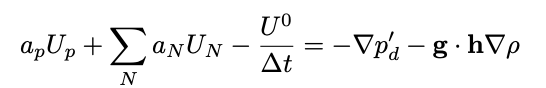
\includegraphics[scale=0.8]{disc}
\end{figure}

//(I will write my own derivation with my own pictures during the christmas break) \\
\vspace{\baselineskip}
Since $a_p U_p = AU$ and \[ \sum_{n=1} a_N U_N - \frac{U^0}{\delta t} = -H \], together with the fact that AU - H = MU, we get that MU = -$\nabla p$.
\vspace{\baselineskip}
After the pressure has been calculated, the density is calculated using the continuity equation. Then the new pressure is used to calculate a new U vector, by setting
\begin{verbatim}
    U = HbyA - RAU*fvc::grad(p);
\end{verbatim}
Constraints are enforced, the pressure is corrected and the kinetic energy K is adjusted. Next limits for pressure are checked, and lastly, unless dpdt is turned off (in the thermophysical properties file) the dpdt term is calculated.

\section{EEqn}

.../reactingFoam/EEqn.H:
\begin{verbatim}
    {
     volScalarField& he = thermo.he();
 
     fvScalarMatrix EEqn
     (
         fvm::ddt(rho, he) + mvConvection->fvmDiv(phi, he)
       + fvc::ddt(rho, K) + fvc::div(phi, K)
       + (
             he.name() == "e"
           ? fvc::div
             (
                 fvc::absolute(phi/fvc::interpolate(rho), U),
                 p,
                 "div(phiv,p)"
             )
           : -dpdt
         )
       - fvm::laplacian(turbulence->alphaEff(), he)
      ==
         reaction->Qdot()
       + fvOptions(rho, he)
     );
 
     EEqn.relax();
 
     fvOptions.constrain(EEqn);
 
     EEqn.solve();
 
     fvOptions.correct(he);
 
     thermo.correct();
 
     Info<< "min/max(T) = "
         << min(T).value() << ", " << max(T).value() << endl;
 }
\end{verbatim}

Assuming we are using the enthalpy energy equation, where he.name() == "h" and therefore the fifth term being equal to dpdt, we can set up the equation in the following way:

\begin{figure}[H]
\centering
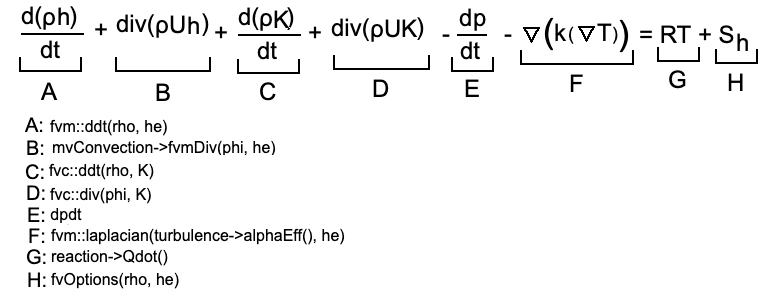
\includegraphics[scale=0.4]{energycode}
\end{figure}

Where RT is the temperature gained from chemical reactions.
Since $h_0 = h + K$ we have $\frac{d \rho h}{dt} + \frac{d \rho K}{dt} = \frac{d \rho h_0}{dt}$ and $div(h) + div(K) = div(h_0)$
\vspace{\baselineskip}
Moving the -dpdt term and the diffusive term to the RHS we get:

\begin{figure}[H]
\centering
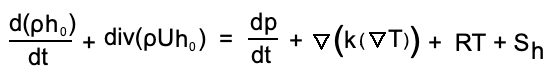
\includegraphics[scale=0.6]{energycode2}
\end{figure}

This is similar to the total enthalpy equation in the book:
\begin{figure}[H]
\centering
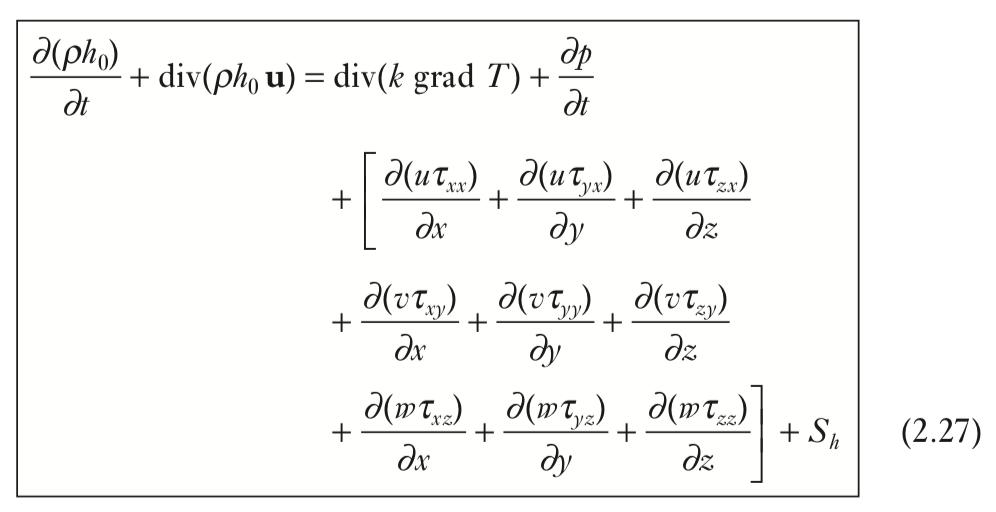
\includegraphics[scale=0.5]{enthalpytot}
\end{figure}
except that the dissipation term has been ignored and we have an extra reaction term RT.
\vspace{\baselineskip}
$\frac{dK}{dt}$ and div(K) are calculated explicitly since they only depend on the U matrix which is already solved in UEqn.H. The diffusive term depends on temperature which is solved alongside the enthalpy, and therefore needs to be solved implicitly.

\section{YEqn}

.../reactingFoam/YEqn.H:
\begin{verbatim}
 tmp<fv::convectionScheme<scalar>> mvConvection
 (
     fv::convectionScheme<scalar>::New
     (
         mesh,
         fields,
         phi,
         mesh.divScheme("div(phi,Yi_h)")
     )
 );
 
 {
     reaction->correct();
     volScalarField Yt(0.0*Y[0]);
 
     forAll(Y, i)
     {
         if (i != inertIndex && composition.active(i))
         {
             volScalarField& Yi = Y[i];
 
             fvScalarMatrix YiEqn
             (
                 fvm::ddt(rho, Yi)
               + mvConvection->fvmDiv(phi, Yi)
               - fvm::laplacian(turbulence->muEff(), Yi)
              ==
                 reaction->R(Yi)
               + fvOptions(rho, Yi)
             );
 
             YiEqn.relax();
 
             fvOptions.constrain(YiEqn);
 
             YiEqn.solve("Yi");
 
             fvOptions.correct(Yi);
 
             Yi.max(0.0);
             Yt += Yi;
         }
     }
 
     Y[inertIndex] = scalar(1) - Yt;
     Y[inertIndex].max(0.0);
 }
\end{verbatim}

inertIndex represents the index for inert mass, i.e. the fluid molecules that are not explicit components in any reaction, but might act as energy receptors for the reactions of other molecules. In this case, it will represent all molecules found in air except $OH, CH_4, O_2, O_3, NO and NO_2$.
\vspace{\baselineskip}
Yi represents the mass fraction of a certain species, that is $\frac{\rho_i}{\rho}$.
\vspace{\baselineskip}
Setting up the equation:

\begin{figure}[H]
\centering
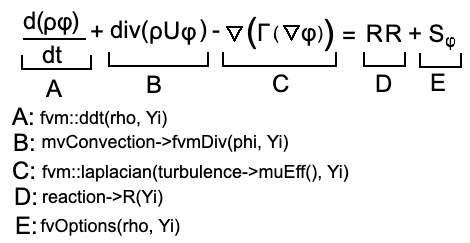
\includegraphics[scale=0.8]{transportcode}
\end{figure}

We can easily see how it resembles the scalar transport equation from the book:
\begin{figure}[H]
\centering
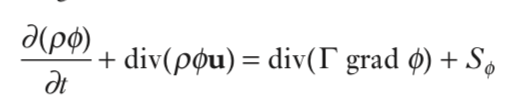
\includegraphics[scale=0.7]{transport}
\end{figure}
The only difference is the reaction->R(Yi) term, which represents the reaction source RR.

